\chapter{\textit{Dataset} da Competição: Produção Energética e Sustentabilidade}

\section{Descrição}
\paragraph{}
O \textit{dataset} de competição, é um cojunto de \textit{datasets} disponibilizados pela equipa docente, apresentando diversos dados referentes à produção energética de determinados painéis solares e à situação meteorológica na cidade de Braga, para cada hora e dia do ano de 20021 até ao ano de 2023.
Os \textit{datasets} utilizados nesta competição contêm um elevado conjunto de \textit{features} sendo de destacar a \textit{feature} Injeção na rede (kWh). Esta \textit{feature} é considerada o nosso target, uma vez que, o problema que se impõe, com estes \textit{datasets}, é prever a quantidade de energia, em kWh, produzida por painéis e injetada, em redes elétricas, a cada hora do dia. 

\section{Exploração de dados}

\subsection{Tipos de dados}
\paragraph{}
Através da método \textit{info()}, conseguimos verificar o tipo de cada coluna, sendo possível identificar 5 colunas do tipo \textit{object} (Data, Injeção na rede (kWh), dt\_iso, city\_name e weather\_description), que serão tido em conta na preparação de dados para poderem ser utilizados nos modelos criados.

\begin{figure}[H]
    \centering
    \centerline{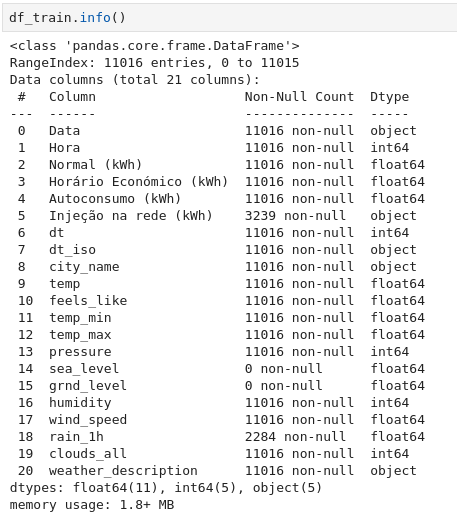
\includegraphics[width=0.5\textwidth]{Imagens/Competição/info_competicao.png}}
    \caption{Método \textit{info()}}
    \label{fig: info_competicao}
\end{figure}

\subsection{\textit{Missing values}}
\paragraph{}
Na análise dos dados foi verificada a existência de \textit{missing values} nos dados de treino nas colunas Injeção na rede (kWh), sea\_level, grnd\_level e rain\_1h. Já nos dados de teste para além destas últimas 3 colunas, os dados que acrescentamos apresentavam \textit{missing values} nas colunas temp\_min e temp\_max.

\begin{figure}[H]
    \centering
    \centerline{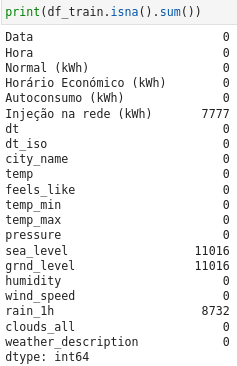
\includegraphics[width=0.3\textwidth]{Imagens/Competição/missing_values.png}}
    \caption{\textit{Missing values}}
    \label{fig: missing_values}
\end{figure}


\section{Preparação de dados}

\subsection{\textit{Feature} engeneering sobre as datas}
\paragraph{}
Através da coluna 'Data' o grupo aplicou técnicas de \textit{feature} engineering para extrair novas \textit{features} a partir desta. A partir desta retiramos então o ano, mês e dia com o objetivo de verificar se algum destes atributos tinha influência na nossa \textit{label}.

\subsection{Tratamento de \textit{missing values}}
\paragraph{}
Para os \textit{missing values} de Injeção na rede (kWh) e rain\_1h o grupo considerou que a falta de valores nas colunas deve-se ao facto de não ter havido injeção na rede ou chuva, deste modo todos os valores em falta foram preenchidos com valor 0 para representar a inexistência de injeção ou chuva.
Já para as \textit{features} sea\_level, grnd\_level, uma vez que toda a coluna apresentava \textit{missing values} decidimos remover ambas as colunas uma vez que, as mesmas, não acrescentam informação importante para treinar os nossos modelos.

Removemos ainda as colunas 'dt' e 'dt\_iso', uma vez que sendo um valor distinto para cada linha, não representa nenhuma informação relevante para o treino dos nossos modelos. Pela razão oposta foi também retirada a \textit{feature} city\_name por ser um valor único para todas as linhas e, por essa razão, não representar informação relevante para o treino dos nossos modelos.

\subsection{Tratamento de dados categóricos}
\paragraph{}
Para tratamento do dados categóricos restantes, weather\_description e Injeção na rede (kWh), visto que ambas as colunas têm uma certa ordem (categóricos ordinais), os valores de ambas as colunas foram substituídos por números inteiros relacionados com a sua ordem prévia.
As associações utilizadas podem ser observadas na seguinte imagem:

\begin{figure}[H]
    \centering
    \begin{minted}[fontsize=\footnotesize, xleftmargin=16pt, breaklines=true, breakanywhere=true]{python}
replace_map = {'Injeção na rede (kWh)': {'None': 0, 'Low': 1, 'Medium': 2, 'High': 3, 'Very High': 4}}
    \end{minted}
    \caption{\textit{Label 'Injeção na rede'}}
    \label{fig1}
\end{figure}

\begin{figure}[H]
    \centering
    \begin{minted}[fontsize=\footnotesize, xleftmargin=16pt, breaklines=true, breakanywhere=true]{python}
replace_map = {'weather_description': {'sky is clear': 1,'few clouds': 2, 'scattered clouds': 3,'broken clouds': 4,'overcast clouds': 5, 'light rain': 6, 'moderate rain': 7, 'heavy intensity rain': 8}}
    \end{minted}
    \caption{\textit{Feature 'weather description'}}
    \label{fig2}
\end{figure}

Foram removidos os atributos 'date\_day' e 'date\_year' por não apresentarem uma correlação relevante com nenhuma das restantes \textit{features}, não acrescentando qualquer informação pertinente ao treino dos modelos.
A \textit{feature} 'weather\_description' foi removida por apresentar uma correlação forte com o atributo 'clouds\_all', decidimos manter esta última por apresentar os valores originais sem nenhum tratamento específico, sendo mantido assim a naturalidade dos dados.

Através do \textit{lineplot} que relaciona a hora com a nossa \textit{target}, o grupo decidiu criar um novo atributo que representasse a fase do dia, isto porque a injeção na rede varia consoante a hora do dia. Esta nova coluna foi criada analisando este gráfico:

\begin{figure}[H]
    \centering
    \centerline{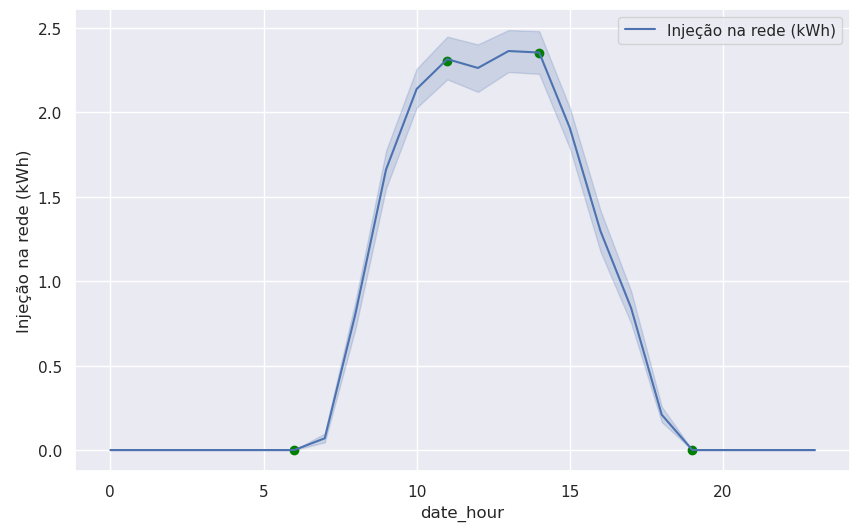
\includegraphics[width=1\textwidth]{Imagens/Competição/line_plot_competicao.png}}
    \caption{Relação da \textit{feature Injeção na Rede} com a \textit{feature date\_hour}}
    \label{fig}
\end{figure}

E com auxilio da seguinte função:
\begin{minted}[fontsize=\footnotesize, xleftmargin=16pt, breaklines=true, breakanywhere=true]{python}
def fase_do_dia(hour):
    if hour <= 6 and hour >= 19:
        return 1
    elif hour <= 11 and hour >= 6:
        return 2
    elif hour <= 14 and hour >= 11:
        return 3
    else:
        return 4
\end{minted}

\section{Modelação}
\paragraph{}
Finalmente, após uma exploração e preparação de dados cuidadosa, partimos então para a criação dos nossos modelos. Para a criação de bons modelos com o objetivo que estes realizassem boas previsões tantos para o nosso \textit{dataset} como para dados desconhecidos, o grupo tentou evitar tanto situações de underfitting como overfitting.
Com este fim o grupo decidiu dividir os dados de treino em 2 conjuntos distintos, um para treinar os modelos e outro para os testar. Foi decidido então que a percentagem de cada um seria 80\% e 20\% respetivamente.

\begin{minted}[fontsize=\footnotesize, xleftmargin=16pt, breaklines=true, breakanywhere=true]{python}
X = df_train.drop(['Injeção na rede (kWh)'], axis=1)
y = df_train['Injeção na rede (kWh)']
\end{minted}

\begin{minted}[fontsize=\footnotesize, xleftmargin=16pt, breaklines=true, breakanywhere=true]{python}
X_train_p, X_test_p, y_train_p, y_test_p = train_test_split(X, y, test_size=0.2, random_state=2023)
\end{minted}

Sabendo que o problema em mão é de classificação foram criados então os seguintes modelos:

\subsection{Árvores de Decisão}
\paragraph{}
Com o primeiro modelo criado decidimos utilizar Decision Tree, uma vez que foi um dos primeiros modelos abordados durante esta UC. Para além disso são também um dos modelos mais usados perante problemas de classificação.

Numa perspetiva mais de programação, foi utilizado DecisionTreeClassifier presente na biblioteca Sklearn e para obter os melhores hiperparâmetros, recorremos ao auxílio de GridSearchCV.

\begin{minted}[fontsize=\footnotesize, xleftmargin=16pt, breaklines=true, breakanywhere=true]{python}
param_grid_dt = { 'criterion': ['gini','entropy','log_loss'], 'max_depth': [5,6,7,8], 'min_samples_split': [2,3,4], 'min_samples_leaf': [1,2,3,4] }
estimator_dt = DecisionTreeClassifier(random_state=2021)
grid_dt = GridSearchCV(estimator_dt, param_grid_dt, refit=True, verbose=0)
\end{minted}

O melhor modelo obtido foi:
\begin{figure}[H]
    \centering
    \centerline{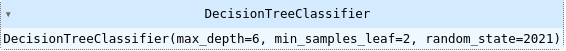
\includegraphics[width=0.7\textwidth]{Imagens/Competição/dt.png}}
    \label{fig: dt}
\end{figure}

e feita a previsão para os dados de teste criados foi obtido então uma accuracy de 86.66\%. Através do classification report analisamos ainda outras métricas como f1-score e recall.

\subsection{Random Forest}
\paragraph{}
De seguida decidimos utilizar Random Forest, algoritmo que tínhamos já utilizado durante a licenciatura e foi também abordado no final desta UC como técnica de ensemble learning.
O benefício que estas trazem relativamente às árvores de decisão, é que as random forest têm uma tendência inferior a overfitting sendo um dos aspetos que pretendemos atenuar.

Usamos então RandomForestClassifier e, mais uma vez, com o auxílio de GridSearchCV descobrimos os melhores hiperparâmetros.

\begin{minted}[fontsize=\footnotesize, xleftmargin=16pt, breaklines=true, breakanywhere=true]{python}
param_grid_dt2 = { 'n_estimators': [150,200,250], 'max_depth': [7,8,9], 'min_samples_split': [2,3,4], 'min_samples_leaf': [1,2,3] }
estimator_dt2 = RandomForestClassifier(bootstrap=False, random_state=2022)
grid_dt2 = GridSearchCV(estimator_dt2, param_grid_dt2, refit=True, verbose=0)
\end{minted}

O melhor modelo obtido apresenta os seguintes hiperparâmetros:
\begin{minted}[fontsize=\footnotesize, xleftmargin=16pt, breaklines=true, breakanywhere=true]{python}
{'max_depth': 9, 'min_samples_leaf': 1, 'min_samples_split': 3, 'n_estimators': 150}
\end{minted}

Feita a previsão para o os dados de teste criados obtemos 88.61\% accuracy, um resultado visivelmente melhor que o anteriormente obtido.
Estas melhorias são também visíveis nas métricas disponibilizadas por classification report.
Concluímos então que a random forest generaliza melhor que as decision tree, porém são modelos que requerem um custo computacional mais elevado.

\subsection{Máquinas de Vetores de Suporte (SVM)}
\paragraph{}
Decidimos ainda explorar SVM, para ver como se comportavam perante o nosso \textit{dataset}.
Como nos anteriores modelos foi utilizado GridSearchCV para descobrir os melhores hiperparâmetros do SVC.

O melhor modelo obtido apresenta então os seguintes hiperparâmetros:
\begin{minted}[fontsize=\footnotesize, xleftmargin=16pt, breaklines=true, breakanywhere=true]{python}
param_grid = {'C': [0.1,1,10,100,1000], 'gamma': [1,0.1,0.01,0.001,0.0001], 'kernel': ['rbf','linear']}
\end{minted}

E os seguintes resultados:
\begin{minted}[fontsize=\footnotesize, xleftmargin=16pt, breaklines=true, breakanywhere=true]{python}
{'C': 1000, 'gamma': 0.001, 'kernel': 'rbf'}
\end{minted}

Como já esperávamos este modelo foi o que nos trouxe uma accuracy inferior no entanto conseguiu prever 85.66\% dos valores corretos.

\subsection{XGBoost}
\paragraph{}
Uma vez lecionada, procedemos à implementação de novas técnicas de ensemble learning procedendo à implementação de XGBoost.

Mais uma vez utilizamos GridSearchCV para descobrir os melhores hiperparâmetros para XGBClassifier.
\begin{minted}[fontsize=\footnotesize, xleftmargin=16pt, breaklines=true, breakanywhere=true]{python}
param_xgb = {'n_estimators': [200,225,250], 'learning_rate': [0.05,0.1,0.2], 'max_depth': [3,4,5]}
estimator_xgb = XGBClassifier()
grid_xgb = GridSearchCV(estimator_xgb, param_xgb, scoring='accuracy', refit=True, verbose=0)
\end{minted}

O melhor modelo obtido apresenta então os seguintes hiperparâmetros:
\begin{minted}[fontsize=\footnotesize, xleftmargin=16pt, breaklines=true, breakanywhere=true]{python}
{'learning_rate': 0.05, 'max_depth': 5, 'n_estimators': 225}
\end{minted}

Este modelo apresentou a melhor accuracy de todos os modelos de cerca de  89.11\%.

\subsection{Stacking}
\paragraph{}
Por fim aplicamos stacking recorrendo a todos os modelos criados durante esta fase, para assim aproveitar as forças individuais de todos os modelos criados, combinando as previsões obtidas de maneira ponderada.

O modelo utilizado foi então:
\begin{minted}[fontsize=\footnotesize, xleftmargin=16pt]{python}
estimators = [('dt', dt_model), ('svm', svm_model), ('rf', rf_model), ('xgb', xgb_model)]
\end{minted}

\begin{minted}[fontsize=\footnotesize, xleftmargin=16pt, breaklines=true, breakanywhere=true]{python}
st_model = StackingClassifier(estimators = estimators, final_estimator = LogisticRegression(max_iter=1000))
\end{minted}

Obtemos então uma accuracy de 88.97\%

\section{Avaliação}
\paragraph{}
Como vimos, foram criados e testados vários modelos durante a fase de modelagem. Foi determinado pelo grupo que o modelo a utilizar para previsão dos dados de teste fornecido pela equipa docente seria o último modelo criado recorrendo a stacking. Embora não tenha sido o modelo que obteve melhor accuracy perante os nossos dados consideramos que por considerar vários resultados obtidos de outros modelos previamente criados, este se encontra melhor preparado para dados desconhecidos.

A accuracy final que foi obtida com este modelo foi de 87.09\% no leaderboard privado, ficando na posição número 18. Perante estes resultados podemos afirmar que o nosso modelo tem um comportamento aceitável perante dados desconhecidos e não tem tendência para overfitting, sendo os pontos que mais tivemos em atenção na criação dos modelos.

Deste modo, embora estejamos satisfeitos com os resultados obtidos, visto a nossa classificação final pensamos que poderíamos ter efetuado algumas melhorias, como por exemplo uma melhor exploração de dados e criação de novos modelos.
